\section{Preliminaries}
\label{sec:perliminary}

\begin{figure}[tbp]
	\hspace{0ex}
	\vspace{0ex}
	\centering
	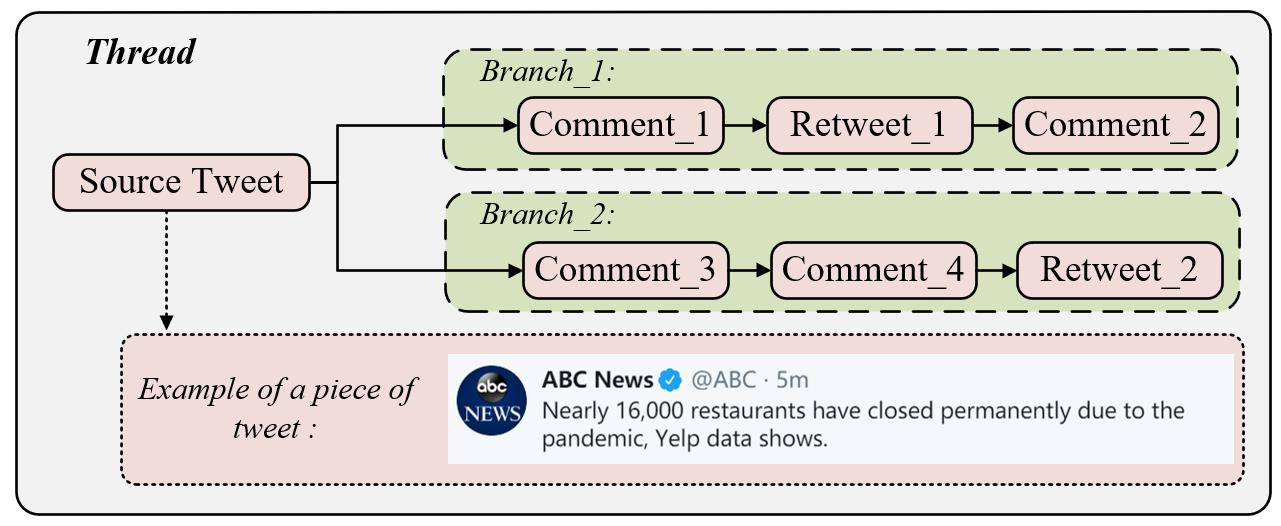
\includegraphics[width = \textwidth]{fig/data_format}
	\caption{An Overview of Social Network Data}
	\label{fig:data_format}
\end{figure}

In this section, we will introduce the essential notations, problem definitions, and background knowledge of rumor tracking. The frequently used notations are summarized in Table.~\ref{tab:notations}.

\subsection{Social Network Data}
\label{sec:social_network_data}
We use benchmark dataset PHEME\cite{DBLP:conf/coling/KochkinaLZ18} and RumorEval\cite{DBLP:conf/semeval/EnayetE17} from twitter. The data format is shown in Fig.\ref{fig:data_format}. As we can see, a tweet thread is a source tweet with all its retweets and comments. These retweets and comments are from several branches, which seems like a tree structure. A tweet branch consists of a series of tweets. For a tweet, it contains various types of features, including content, publication time, screen name, etc. The statistical details are shown in Table\ref{tab:pheme} and Table\ref{tab:RumorEval}.


\begin{table}[hbp]
	\caption{Notation Summarization}
	\centering
	\label{tab:notations}
	\resizebox{0.9\linewidth}{!}{
		\begin{tabular}{|c|l|c|l|}
			\hline
			\textbf{Notation} & \textbf{Definition} & \textbf{Notation}& \textbf{Definition}\\
			\hline
			$T$ & the set of tweets & $y_F'$ & output of FastText \\
			\hline
			$t_n$ & a tweet&$y_T'$ & output of TextCNN\\
			\hline
			$C$ & the set of rumor events&$y_B'$ & output of BiLSTM\\
			\hline
			$c_m$ & a rumor event&$y_N'$ & output of Naive Bayes\\
			\hline
			$r$ & predictable result of a component&$y_S'$ & output of SGD\\
			\hline
			$R$ & predictable result of ART& $y'$& output of the ART\\
			\hline
			$x \in R^d$ & a processed sample& $K_y$& set of all components outputs\\
			\hline
			$y \in R^m$ & a training label&&\\
			\hline						
		\end{tabular}
	}	
\end{table}

\subsection{Problem Definition}
\label{sec:problem}
Let $T = \left\{t_1, t_2, ..., t_n \right\}$ denote the set of tweets and each tweet is denoted as $t_n$. Let $C = \left\{c_1, c_2, ... , c_m \right\}$ denote the set of rumor events and $c_m$ denotes a particular rumor event. Each tweet is only assigned with one rumor event. For each given tweet $t_n$, the goal of rumor tracking is to find the most likely relevant event of it. In this work, we transfer the binary rumor tracking problem (related/irrelated) into an m-way classification problem. By preprocessing, the dataset is transformed into: $$\left\{ (x^{(1)}, y^{(1)}), (x^{(2)}, y^{(2)}),..., (x^{(n)}, y^{(n)}) \right\}, x^{(i)} \in R^d, y^{(i)} \in R^m $$ And we denote the output as $y'$. Since the ART is an aggregated model, the optimization goal of each component is different. We denote the predictable result of a component as $r$ and the predictable result of the ART as $R$. Also, for a testing sample, we will not get any information about its branch or threads in advance. 

However, source tweets in the dataset are collected by keywords of the event, which causes the source tweets in the same thread are highly similar to each other. We conduct an experiment to train a classifier on source tweets and the classification result even reaches 100\%. Consequently, we should process each tweet independently and cut down its link to source tweet. Only in this way, we can get a convincing result. 

\subsection{Basic Models for Text Classification}
\label{sec:deeplearning_model} There are several basic models achieving great success on text classification tasks.  In this work, we adopt some effective models as the components of ART. Then we will introduce some of them.

\subsubsection{Machine Learning based Model}
\textbf{Naive Bayes} is a classical classifier. It assumes that all input variables are independent of each other. Although this model is not complicated, it can achieve a satisfying accuracy with high efficiency. Naive Bayes model is widely adopted in the short text classification problem, showing a pretty good performance. The procedure of Naive Bayes is denoted as following:
\begin{align}\label{eq:nb}
y_{N_{i}}' &= \frac{P(y_i)\prod_{j = 0}^d P(x_j|y_i)}{\prod_{j = 0}^d P(x_j)},\\
y_N' &= concat(y_{N_{1}}',y_{N_{2}}',..., y_{N_{i}}'),
\end{align}
where $x_j$ is a dimension of $x$, corresponding to a word in tweet.  $y_i$ is a dimension of training sample $y$. $y_{N_{i}}'$ is a dimension of $y_N'$, representing the probability of a classification. $y_N'$ is the final output of Naive Bayes component.

\textbf{SGD} is the abbreviation of stochastic gradient descent, which is an optimization strategy in deep learning. SGD updates parameters of a single sample, so SGD works well on the dataset on a large scale. We denote the procedure of SGD as $S()$, and the output of SGD components is:
\begin{equation}\label{eq:sgd}
y_S' = S(TFIDF(x)),
\end{equation}
where TFIDF is Term Frequency-Inverse Document Frequency. Finally, the $y_S'$ represents the final output of SGD.

\subsubsection{Deep Learning based Model}
\textbf{BiLSTM} is Bi-directional Long Short-Term Memory, which is consisted of a forward-LSTM and a backward-LSTM. BiLSTM can effectively learn the long term dependency of sequential data. So we usually treat it as a evolution of LSTM and it is suitable for text data. The details of BiLSTM are following:
\begin{align}\label{eq:lstm}
x_tL/R &= Embedding(x_tL/R), \\
x_t &= concat(x_tL, x_tR), \\
i_t &= \sigma(W_i \cdot [h_{t-1}, x_t] + b_i),\\
f_t &= \sigma(W_f \cdot [h_{t-1}, x_t]),\\
\widetilde{C_t} &= tanh(W_{\tilde{C_t}} \cdot [r_t C_{t-1}, x_t]  + b_C),\\
C_t &= (1-f_t) C_{t-1} + f_t \widetilde{C_t},\\
h_t &=o_t \* \tanh(C_t),\\
y_B^{'} &= o_t =  \sigma(W_o \cdot h_t),
\end{align}
where $x_t$ is the input at time step $t$, and it is concatenated by leftward unit $x_tL$ and rightward unit $x_tR$. BiLSTM consists of three gates: forget gate $f_t$, input gate $i_t$, and output gate $o_t$. Also, it has two memories: long-term memory $C_t$ and short-memory $h_t$. Finally, we use output $o_t$ as the final output of BiLSTM, denoted as $y_B^{'}$.

\textbf{FastText} is proposed in 2017 \cite{DBLP:journals/tacl/BojanowskiGJM17, DBLP:journals/corr/JoulinGBDJM16, DBLP:conf/eacl/GraveMJB17}, which is an extension of the skip-gram model introduced by Mikolov et al. \cite{DBLP:conf/nips/MikolovSCCD13}. The main difference between FastText and skip-gram is that the predictable target of FastText is a classification label rather than a middle word. Also, FastText adopts hierarchical softmax to deal with the large corpus and vocabulary dictionary. With the help of these optimizations, FastText classifies large amounts of texts in a short time. For simplicity, we denote the output of FastText as $y_F'$.

\textbf{TextCNN} \cite{DBLP:conf/emnlp/Kim14} uses multiple convolutional filters with different sizes to capture N-gram features. Compared to RNN based models, TextCNN reaches convergence faster due to the parallel computation. The tweets are usually short text (within 140 words) with sparse semantic. Consequently, CNN based models are more suitable than RNN based models for tweets classification where tweets are usually treated as a bag of words. The brief procedure of TextCNN is shown as follows.

\begin{align}\label{eq:tcnn}
V_x &= Embedding(x), \\
m_3 &= maxpooling(ConV_3(V_x)),\\
m_4 &= maxpooling(ConV_4(V_x)),\\
m_5 &= maxpooling(ConV_5(V_x)),\\
y_T' &= flatten(concat(m_3, m_4, m_5)),
\end{align}
where the $Embedding()$ is the embedding layer, and $m$ is the output of different convolutional filters. By concatenating and flattening, the final output of TextCNN component is denoted as $y_T'$.